\section{Unidad 1: Plataforma, arquitectura y conceptos base}

\subsection{ARM y contexto general}

\begin{itemize}
  \item \textbf{ARM:} \textit{Advanced RISC Machines}.
  \item \textbf{Linea de trabajo de la materia:} ARM Cortex-M3.
  \item \textbf{Antecedentes historicos mostrados en clase:}
  \item diseno inicial en 1983;
  \item primer prototipo ARM-1 en 1985;
  \item ARM-2 en 1986.
  \item \textbf{Datos iniciales asociados a esos nucleos:}
  \item bus de datos de 32 bits;
  \item 16 registros de 32 bits;
  \item implementacion muy compacta para su epoca.
  \item \textbf{Idea general:} la familia ARM se usa masivamente en sistemas embebidos y dispositivos portatiles.
\end{itemize}

\subsection{Microcontrolador y placa usados en la materia}

\begin{itemize}
  \item \textbf{Microcontrolador:} LPC1769.
  \item \textbf{Fabricante:} NXP Semiconductors.
  \item \textbf{Familia:} LPC17xx.
  \item \textbf{Nucleo:} ARM Cortex-M3.
  \item \textbf{Frecuencia maxima:} 120 MHz.
  \item \textbf{Flash:} hasta 512 kB.
  \item \textbf{SRAM total:} hasta 64 kB.
  \item \textbf{Placa de desarrollo:} LPCXpresso LPC1769 CMSIS-DAP.
  \item \textbf{Numero de placa:} OM13085.
  \item \textbf{Revision vista en el esquematico:} D1.
  \item \textbf{Interfaz de depuracion integrada:} CMSIS-DAP implementada con un LPC11U35.
  \item \textbf{Conexion principal de la placa:} USB micro-B.
  \item \textbf{Alimentacion mostrada en el esquematico:} USB, +5 V externo y opcion externa de +3.3 V.
  \item \textbf{Conectividad visible en la placa:} conectores de expansion, conector externo de debug y pinout compatible a alto nivel con mbed.
\end{itemize}

\begin{figure}[H]
  \centering
  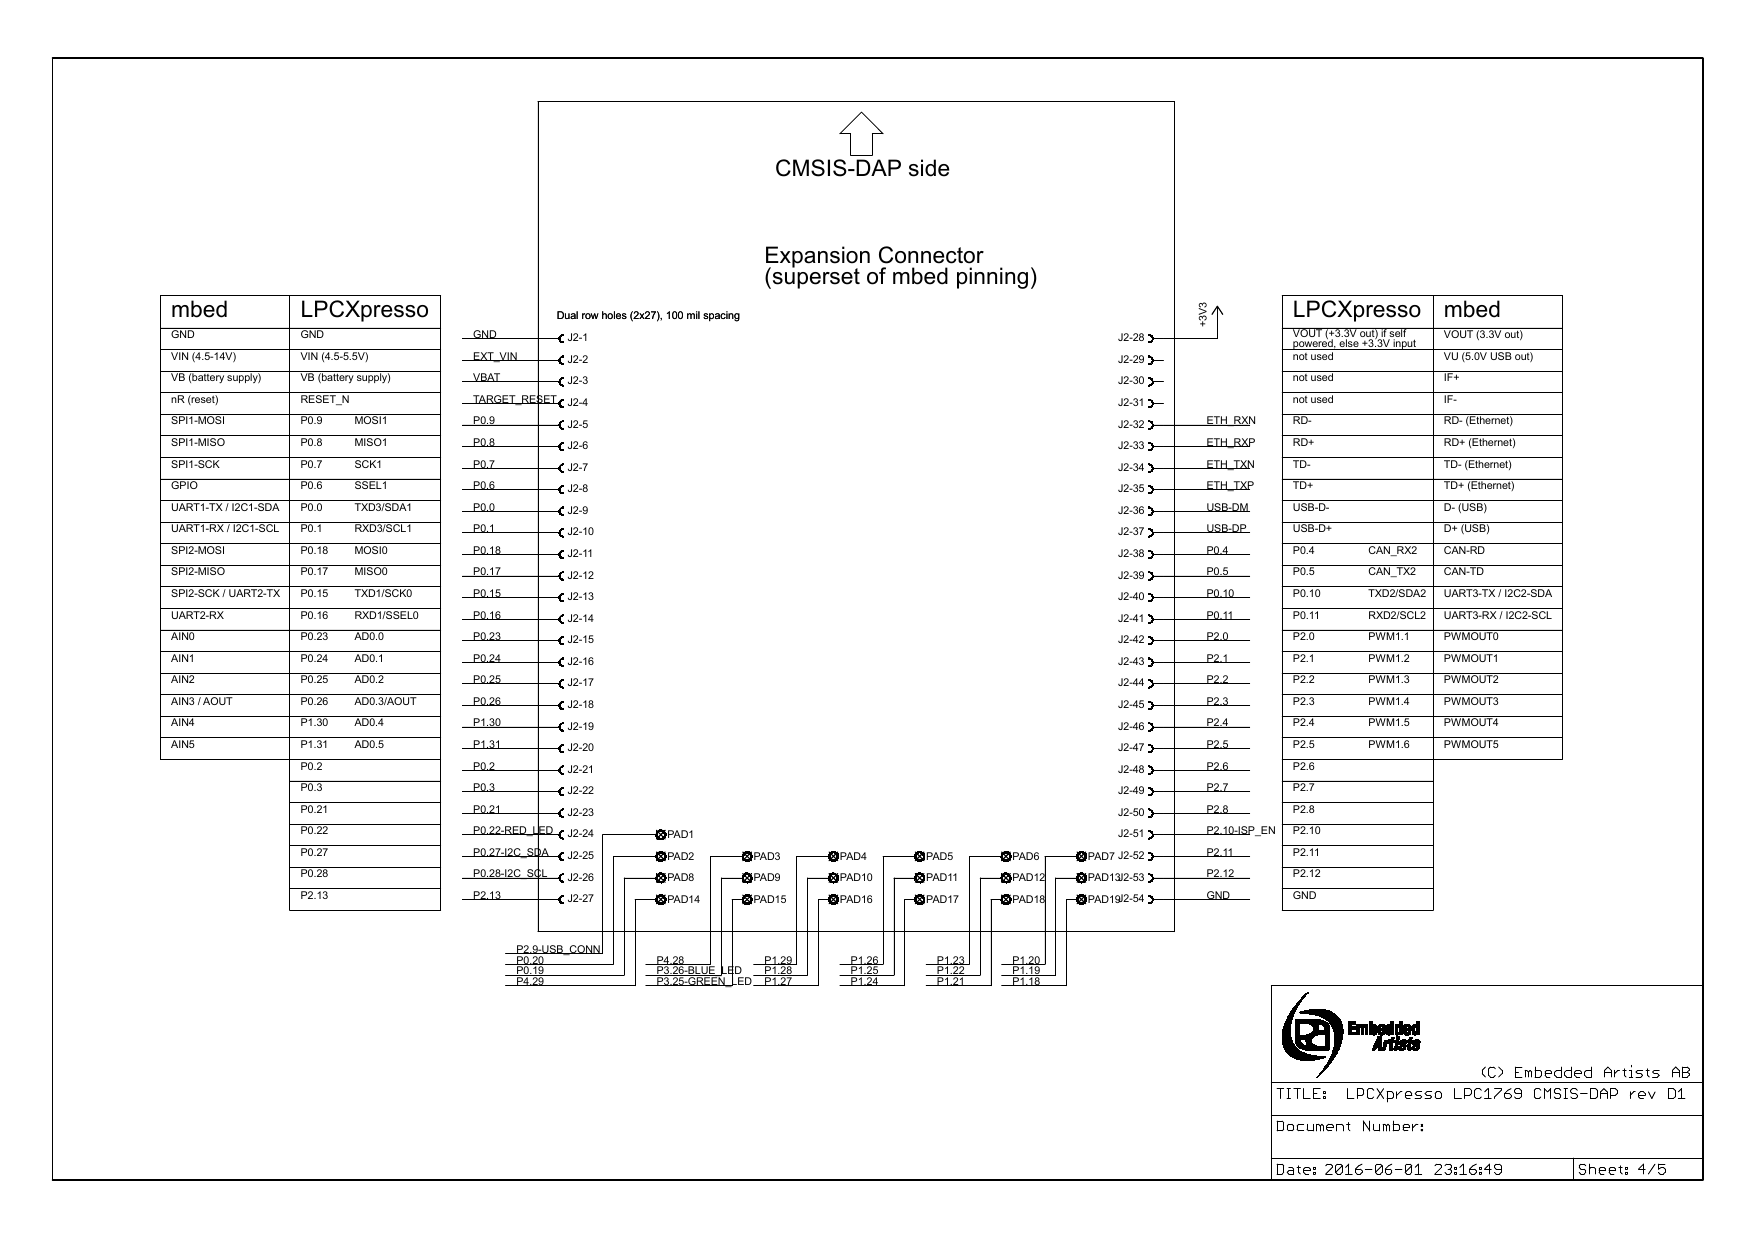
\includegraphics[width=\textwidth,trim=55 40 55 40,clip]{images/placa_lpcxpresso_connector-4.png}
  \caption{Conectores, pines expuestos y relacion entre la placa LPCXpresso y el LPC1769.}
\end{figure}

\subsection{Modelo basico de trabajo en ARM}

\begin{itemize}
  \item ARM procesa datos principalmente en \textbf{registros}.
  \item Las instrucciones operan sobre esos registros.
  \item El acceso a memoria se hace por instrucciones de carga y almacenamiento.
  \item \textbf{Carga:} \texttt{LDR}, de memoria a registro.
  \item \textbf{Almacenamiento:} \texttt{STR}, de registro a memoria.
\end{itemize}

\subsection{Caracteristicas del Cortex-M3 vistas en clase}

\begin{itemize}
  \item \textbf{Arquitectura:} ARMv7-M.
  \item \textbf{MMU:} no posee.
  \item \textbf{Tabla de vectores:} contiene direcciones, no instrucciones.
  \item \textbf{Division:} dispone de instruccion \texttt{DIV}.
  \item \textbf{Interrupciones:} el hardware salva y restaura estado automaticamente.
  \item \textbf{Mapa de memoria:} fijo.
  \item \textbf{Bit-banding:} soportado.
  \item \textbf{NMI:} interrupcion no enmascarable presente.
  \item \textbf{Juego de instrucciones:} compatible con Thumb-2.
\end{itemize}

\subsection{ARM7TDMI, Thumb y Thumb-2}

\begin{itemize}
  \item \textbf{Base de la explicacion de clase:} transicion conceptual de ARM7TDMI hacia Cortex-M3.
  \item \textbf{T:} extension de la arquitectura Thumb.
  \item \textbf{D:} extensiones para depuracion.
  \item \textbf{M:} multiplicador mejorado.
  \item \textbf{I:} \textit{Embedded ICE Macrocell}.
  \item \textbf{ARM de 32 bits:} mas completo en instrucciones y modos de direccionamiento.
  \item \textbf{Thumb de 16 bits:} mas compacto.
  \item \textbf{Thumb-2:} combina compacidad y expresividad, evitando cambios manuales de modo como parte del flujo normal de programacion.
  \item \textbf{Consecuencia practica:} el compilador en C aprovecha ambas variantes del set de instrucciones.
\end{itemize}

\subsection{Buses del sistema}

\begin{itemize}
  \item \textbf{AHB:} \textit{Advanced High-performance Bus}.
  \item \textbf{VPB:} \textit{VLSI Peripheral Bus}.
  \item \textbf{APB:} \textit{Advanced Peripheral Bus}.
\end{itemize}

\subsection{Bloques principales del LPC1769}

La clase muestra el diagrama de bloques simplificado del LPC17xx y conviene retener al menos estos bloques:

\begin{itemize}
  \item nucleo ARM Cortex-M3;
  \item matriz AHB multicapa;
  \item Flash;
  \item SRAM;
  \item ROM;
  \item GPIO de alta velocidad;
  \item control de clocks y potencia;
  \item DMA;
  \item Ethernet;
  \item USB;
  \item RTC;
  \item pin connect block;
  \item ADC;
  \item DAC;
  \item timers;
  \item PWM;
  \item interrupciones externas;
  \item system control.
\end{itemize}

\subsection{Niveles de programacion}

\begin{itemize}
  \item \textbf{Lenguaje maquina:} hoy no se usa como forma practica de trabajo por costo de desarrollo y dificultad de mantenimiento.
  \item \textbf{Ensamblador:} util cuando importa el control fino, el costo de memoria, el tiempo real, o cuando predominan entrada/salida y control sobre calculo.
  \item \textbf{Lenguaje de alto nivel:} adecuado para programas largos, cambios frecuentes y mayor mantenibilidad.
\end{itemize}

\subsection{CMSIS}

\begin{itemize}
  \item \textbf{CMSIS:} \textit{Cortex Microcontroller Software Interface Standard}.
  \item \textbf{Funcion:} capa comun de abstraccion para microcontroladores basados en Cortex.
  \item \textbf{Objetivo:} dar nombres, estructuras e interfaces consistentes para nucleo, perifericos, herramientas y placas.
  \item \textbf{Uso practico en la materia:} acceder a los registros del LPC1769 con nombres estables desde \texttt{LPC17xx.h}.
\end{itemize}

\subsection{Memoria}

\begin{itemize}
  \item \textbf{Espacio de direccionamiento:} plano, de 32 bits.
  \item \textbf{MPU:} opcional, permite definir regiones de acceso.
  \item \textbf{Perifericos:} mapeados en memoria.
  \item \textbf{Arquitectura Harvard:} caminos separados para instrucciones y datos.
  \item \textbf{Bit-band:} regiones especiales para acceso eficiente a bits.
  \item \textbf{Regiones base del mapa de memoria:}
  \item \texttt{0x0000 0000 - 0x1FFF FFFF}: Flash, SRAM local y Boot ROM.
  \item \texttt{0x2000 0000 - 0x3FFF FFFF}: SRAM AHB y GPIO.
  \item \texttt{0x4000 0000 - 0x5FFF FFFF}: perifericos APB y AHB.
  \item \texttt{0xE000 0000 - 0xE00F FFFF}: perifericos privados del Cortex-M3, incluyendo NVIC y SysTick.
\end{itemize}

\begin{figure}[H]
  \centering
  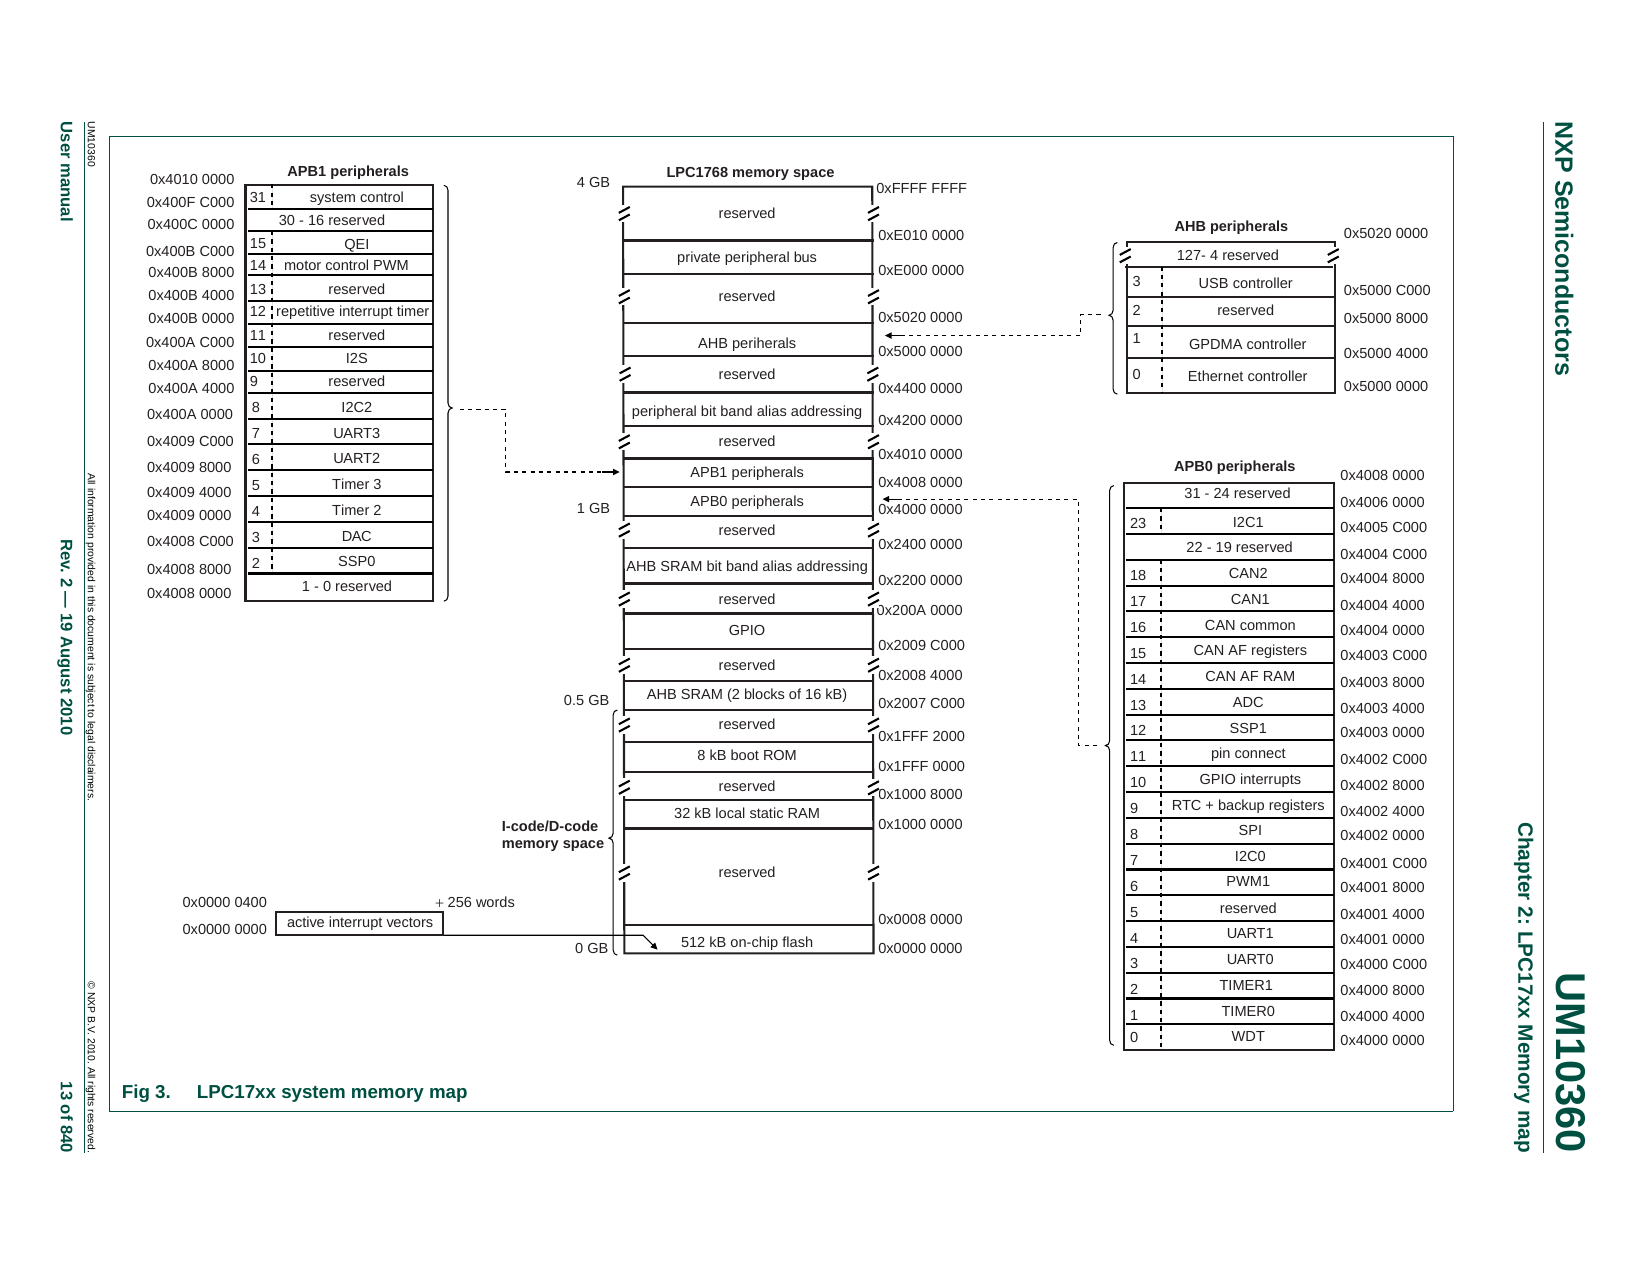
\includegraphics[width=\textwidth]{images/lpc17xx_memory_map_datasheet.png}
  \caption{Mapa de memoria del LPC17xx extraido del datasheet original.}
\end{figure}

\subsection{Caracteristicas electricas}

\textbf{Valores limite}

\small
\renewcommand{\arraystretch}{1.15}
\setlength{\tabcolsep}{4pt}

\begin{longtable}{|>{\raggedright\arraybackslash}p{0.17\textwidth}|>{\raggedright\arraybackslash}p{0.28\textwidth}|>{\raggedright\arraybackslash}p{0.19\textwidth}|>{\centering\arraybackslash}p{0.07\textwidth}|>{\centering\arraybackslash}p{0.07\textwidth}|>{\centering\arraybackslash}p{0.07\textwidth}|}
\hline
\textbf{Simbolo} & \textbf{Parametro} & \textbf{Condiciones} & \textbf{Min} & \textbf{Max} & \textbf{Unidad} \\
\hline
\endfirsthead
\hline
\textbf{Simbolo} & \textbf{Parametro} & \textbf{Condiciones} & \textbf{Min} & \textbf{Max} & \textbf{Unidad} \\
\hline
\endhead
\texttt{VDD(3V3)} & tension de alimentacion (3.3 V) & riel externo & 2.4 & 3.6 & V \\
\hline
\texttt{VDD(REG)(3V3)} & tension de alimentacion del regulador (3.3 V) & & 2.4 & 3.6 & V \\
\hline
\texttt{IDD} & corriente de alimentacion & por pin de alimentacion & -- & 100 & mA \\
\hline
\texttt{ISS} & corriente de tierra & por pin de tierra & -- & 100 & mA \\
\hline
\end{longtable}

\normalsize

\textbf{Caracteristicas estaticas 1}

\textit{Tamb = -40 C a +85 C, salvo indicacion contraria.}

\scriptsize
\renewcommand{\arraystretch}{1.10}
\setlength{\tabcolsep}{3pt}

\begin{longtable}{|>{\raggedright\arraybackslash}p{0.18\textwidth}|>{\raggedright\arraybackslash}p{0.22\textwidth}|>{\raggedright\arraybackslash}p{0.22\textwidth}|>{\centering\arraybackslash}p{0.07\textwidth}|>{\centering\arraybackslash}p{0.07\textwidth}|>{\centering\arraybackslash}p{0.07\textwidth}|>{\centering\arraybackslash}p{0.06\textwidth}|}
\hline
\textbf{Simbolo} & \textbf{Parametro} & \textbf{Condiciones} & \textbf{Min} & \textbf{Tip [1]} & \textbf{Max} & \textbf{Unidad} \\
\hline
\endfirsthead
\hline
\textbf{Simbolo} & \textbf{Parametro} & \textbf{Condiciones} & \textbf{Min} & \textbf{Tip [1]} & \textbf{Max} & \textbf{Unidad} \\
\hline
\endhead
\multicolumn{7}{|l|}{\textbf{Pines de alimentacion}} \\
\hline
\texttt{VDD(3V3)} & tension de alimentacion (3.3 V) & riel externo & 2.4 [2] & 3.3 & 3.6 & V \\
\hline
\texttt{VDD(REG)(3V3)} & tension de alimentacion del regulador (3.3 V) & & 2.4 & 3.3 & 3.6 & V \\
\hline
\texttt{VDDA} & tension de alimentacion analogica de pin (3.3 V) & & 2.7 & 3.3 & 3.6 & V \\
\hline
\texttt{V\_I(VBAT)} & tension de entrada en el pin \texttt{VBAT} & & 2.1 [3] & 3.3 & 3.6 & V \\
\hline
\texttt{V\_I(VREFP)} & tension de entrada en el pin \texttt{VREFP} & & 2.7 & 3.3 & \texttt{VDDA} & V \\
\hline
\end{longtable}

\textbf{Corriente de alimentacion del regulador (3.3 V)}

\begin{longtable}{|>{\raggedright\arraybackslash}p{0.18\textwidth}|>{\raggedright\arraybackslash}p{0.18\textwidth}|>{\raggedright\arraybackslash}p{0.34\textwidth}|>{\centering\arraybackslash}p{0.06\textwidth}|>{\centering\arraybackslash}p{0.07\textwidth}|>{\centering\arraybackslash}p{0.06\textwidth}|>{\centering\arraybackslash}p{0.05\textwidth}|}
\hline
\textbf{Simbolo} & \textbf{Parametro} & \textbf{Condiciones} & \textbf{Min} & \textbf{Tip [1]} & \textbf{Max} & \textbf{Unidad} \\
\hline
\endfirsthead
\hline
\textbf{Simbolo} & \textbf{Parametro} & \textbf{Condiciones} & \textbf{Min} & \textbf{Tip [1]} & \textbf{Max} & \textbf{Unidad} \\
\hline
\endhead
\texttt{I\_DD(REG)(3V3)} & corriente de alimentacion del regulador (3.3 V) & modo activo; codigo \texttt{while(1)\{\}} ejecutado desde flash; todos los perifericos deshabilitados; \texttt{PCLK = CCLK/8} & & & & \\
\hline
 &  & \texttt{CCLK = 12 MHz}; PLL deshabilitado [4][5] & -- & 7 & -- & mA \\
\hline
 &  & \texttt{CCLK = 100 MHz}; PLL habilitado [4][5] & -- & 42 & -- & mA \\
\hline
 &  & \texttt{CCLK = 100 MHz}; PLL habilitado (\texttt{LPC1769}) [4][6] & -- & 50 & -- & mA \\
\hline
 &  & \texttt{CCLK = 120 MHz}; PLL habilitado (\texttt{LPC1769}) [4][6] & -- & 67 & -- & mA \\
\hline
 &  & modo \textit{sleep} [4][7] & -- & 2 & -- & mA \\
\hline
 &  & modo \textit{deep sleep} [4][8] & -- & 240 & -- & uA \\
\hline
 &  & modo \textit{power-down} [4][8] & -- & 31 & -- & uA \\
\hline
 &  & modo \textit{deep power-down}; RTC en ejecucion [9] & -- & 630 & -- & nA \\
\hline
\end{longtable}

\textbf{Corriente de bateria y corriente de E/S}

\begin{longtable}{|>{\raggedright\arraybackslash}p{0.18\textwidth}|>{\raggedright\arraybackslash}p{0.18\textwidth}|>{\raggedright\arraybackslash}p{0.34\textwidth}|>{\centering\arraybackslash}p{0.06\textwidth}|>{\centering\arraybackslash}p{0.07\textwidth}|>{\centering\arraybackslash}p{0.06\textwidth}|>{\centering\arraybackslash}p{0.05\textwidth}|}
\hline
\textbf{Simbolo} & \textbf{Parametro} & \textbf{Condiciones} & \textbf{Min} & \textbf{Tip [1]} & \textbf{Max} & \textbf{Unidad} \\
\hline
\endfirsthead
\hline
\textbf{Simbolo} & \textbf{Parametro} & \textbf{Condiciones} & \textbf{Min} & \textbf{Tip [1]} & \textbf{Max} & \textbf{Unidad} \\
\hline
\endhead
\texttt{I\_BAT} & corriente de alimentacion de bateria & modo \textit{deep power-down}; RTC en ejecucion; \texttt{VDD(REG)(3V3)} presente [10] & -- & 530 & -- & nA \\
\hline
 &  & modo \textit{deep power-down}; RTC en ejecucion; \texttt{VDD(REG)(3V3)} no presente [11] & -- & 1.1 & -- & uA \\
\hline
\texttt{I\_DD(IO)} & corriente de alimentacion de E/S & modo \textit{deep sleep} [12] & -- & 40 & -- & nA \\
\hline
 &  & modo \textit{power-down} [12] & -- & 40 & -- & nA \\
\hline
 &  & modo \textit{deep power-down} [12] & -- & 10 & -- & nA \\
\hline
\end{longtable}

\normalsize
